The results of our main specification are presented in the table \ref{dif_table}, in column (1). The estimated coefficients together with their 95\% confidence  from this model are plotted in the figure \ref{fig_did_effets}. We can see that all coefficients for years 1930 to 1932 are statistically insignificant which means that the pre-treatment trends in arrests of German minority were likely parallel to the pre-treatment trends of other minorities which gives us greater  confidence in the validity of our identification strategy. 

The coefficients on all other years are insignificant as well. Only for 1934 (one year lag) is the estimate  significant at 10\% level ($p$-value of 0.08). Since this not reaches even the traditional 5\% significance threshold we are inclined to not reject the null hypothesis or at least to conclude that evidence in favor of the alternative hypothesis (more repressions of Germans due to rise of Hitler) is quite weak.  Furthermore, as we show below the alternative specifications do not increase the significance of the coefficients.
\begin{figure}[h]
\centering
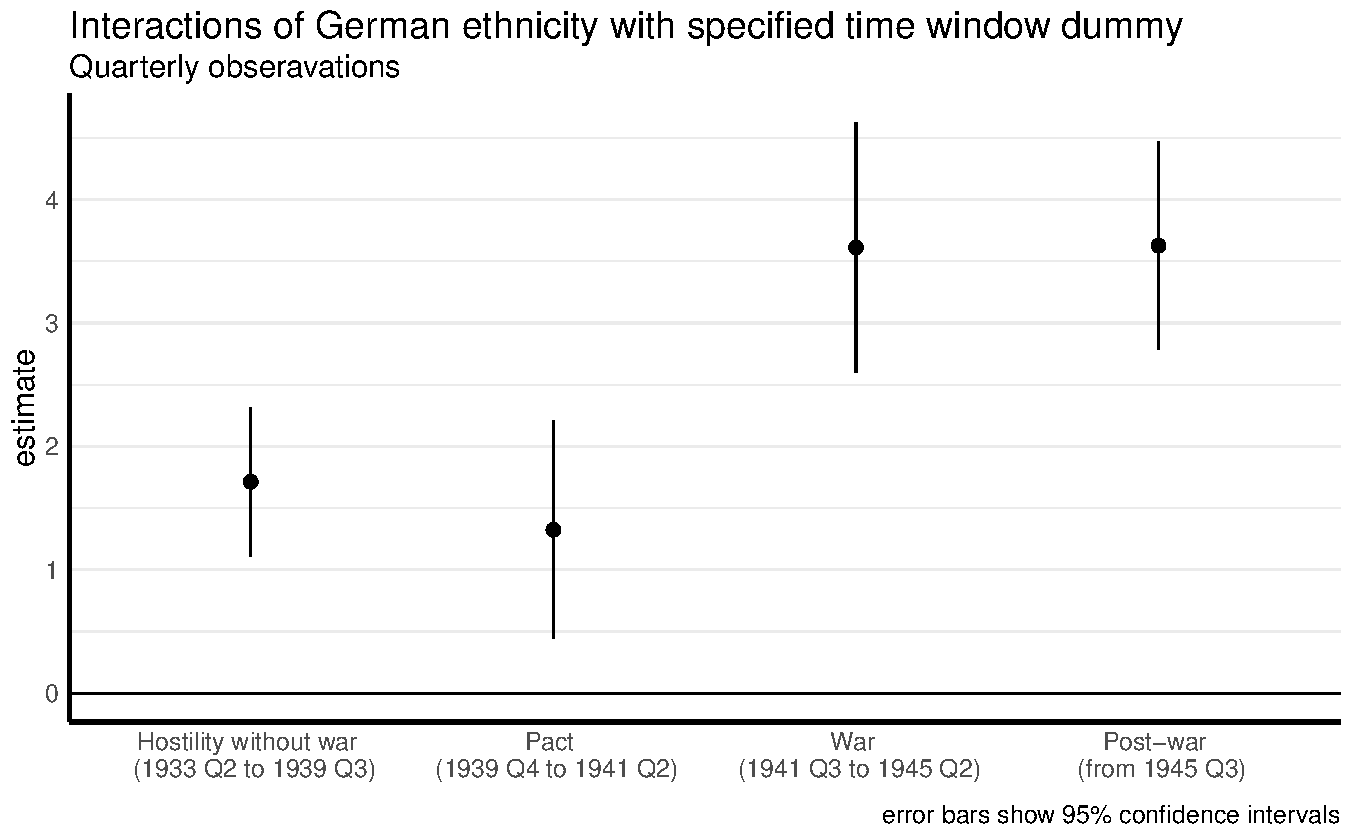
\includegraphics[width=1.1\textwidth]{plots/did_effects_quart_window_postwar.pdf}
\caption{Estimates of coefficients on $german \cdot post\_year$}
\label{fig_did_effets}
\end{figure}
We perform several robustness checks to asses sensitivity of the results to different specifications. First, in our main model (column (1) of table \ref{dif_table}), we included all observations in years 1923 to 1958. But the relationship between Germany and Soviet Union were somewhat more complicated after the World War II. We thus re-estimate the model with only the data from 1923 to 1945. The results (in column (2)) change only little and does not alter our previous conclusions. Second, when we omit the ethnicity specific linear time trends in column (3), we see again that the coefficients are very similar to the original model. 
Finally, we estimate a specification with number of arrests as a dependent variable (without logarithmic transformation). We can see that this model (shown in column (4)) fits the data rather poorly with  $R^2$ only of 0.428 (compared to 0.890 in the logarithmic specification). 